\begin{listing}[H] % Shows source code 1iteratordemo.rb
  \caption{The source code for \emph{1iteratordemo.rb}.}
  \label{lst: source code of 1iteratordemo}
  \inputminted[rulecolor=gray(x11gray),linenos,frame=lines,framesep=5mm]{ruby}{code/1iteratordemo.rb}
\end{listing}
\addcontentssubsection{\textbf{Listing \ref{lst: source code of 1iteratordemo}} Source code for 1iteratordemo.rb} % manually adds this listing to table of contents
\begin{figure}[H] % shows screenshot output of code
  \centering
  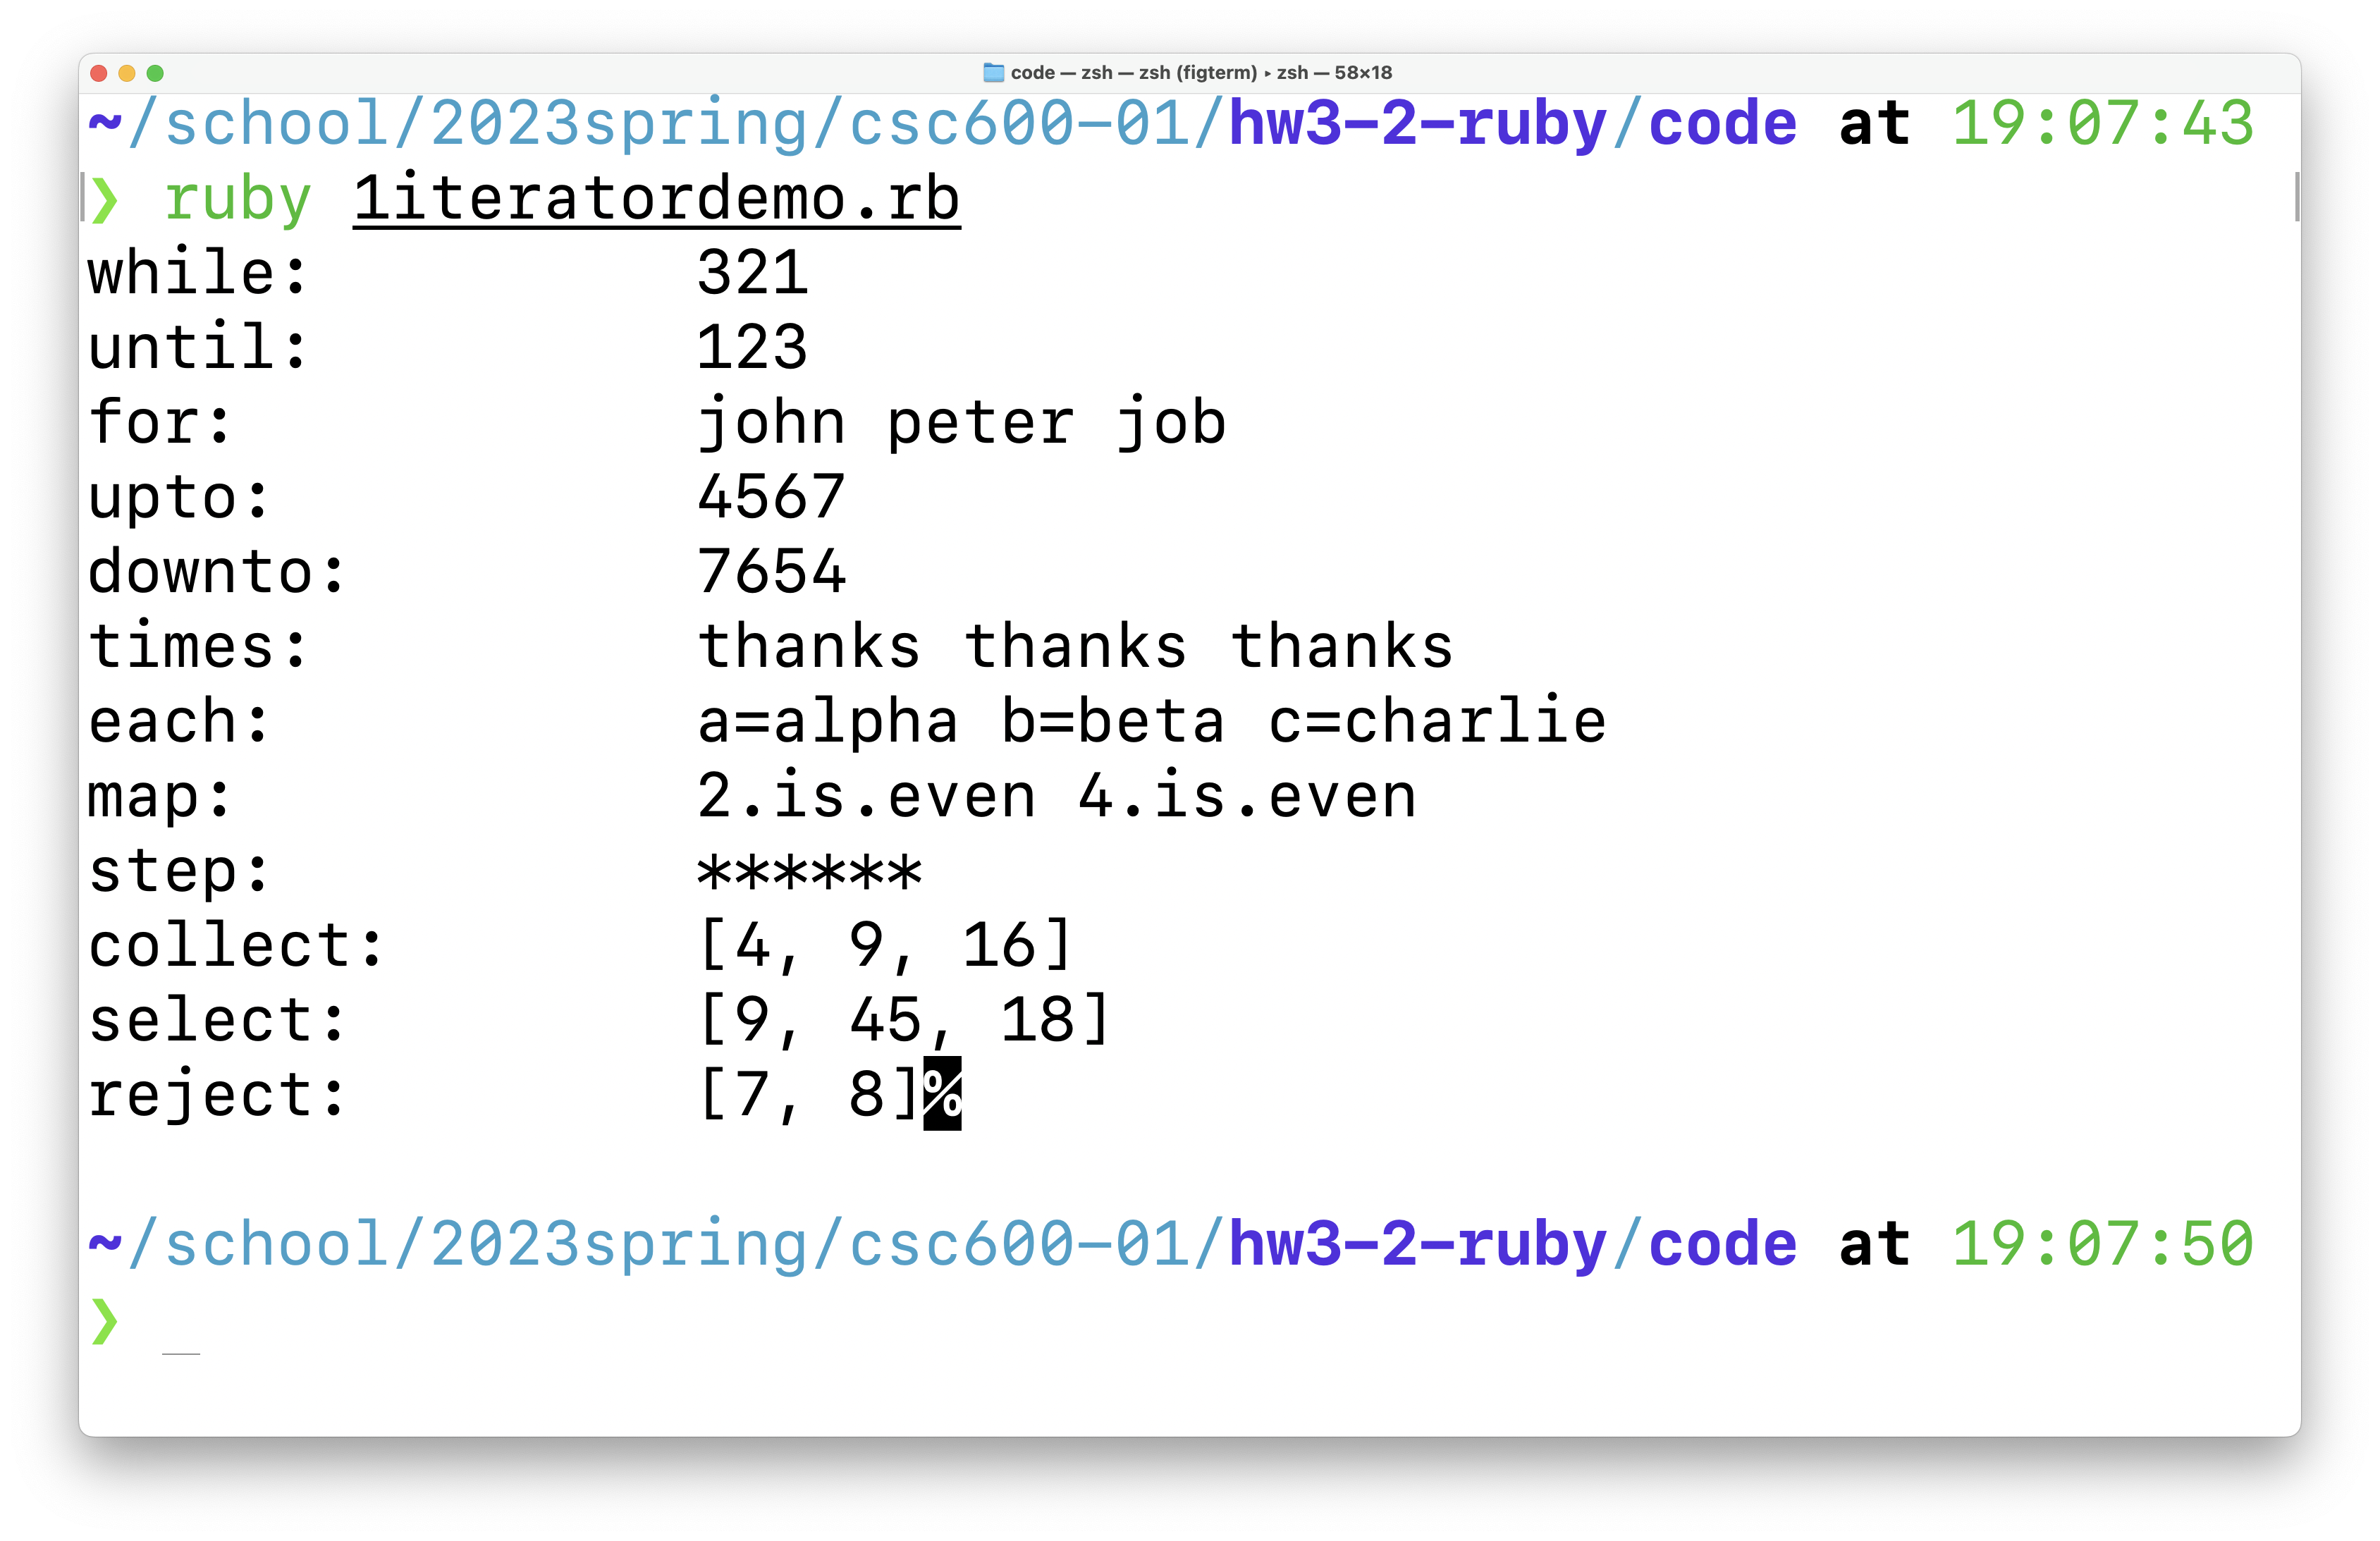
\includegraphics[width=.9\linewidth]{1iteratordemo.PNG}
  \setlength{\captionmargin}{0pt}
  \caption{Screenshot output of executing \emph{1iteratordemo.rb}}
  \label{fig:1iteratordemo.png}
\end{figure}
\addcontentssubsection{\textbf{Figure \ref{fig:1iteratordemo.png}} Screenshot output of executing\emph{1iteratordemo.rb}} % manually adds this listing to table of contents
